
\documentclass[
	% -- opções da classe memoir --
	article,			% indica que é um artigo acadêmico
	11pt,				% tamanho da fonte
	oneside,			% para impressão apenas no verso. Oposto a twoside
	a4paper,			% tamanho do papel. 
	% -- opções da classe abntex2 --
	%chapter=TITLE,		% títulos de capítulos convertidos em letras maiúsculas
	%section=TITLE,		% títulos de seções convertidos em letras maiúsculas
	%subsection=TITLE,	% títulos de subseções convertidos em letras maiúsculas
	%subsubsection=TITLE % títulos de subsubseções convertidos em letras maiúsculas
	% -- opções do pacote babel --
	english,			% idioma adicional para hifenização
	brazil,				% o último idioma é o principal do documento
	sumario=tradicional
	]{abntex2}

\newcommand{\matlabCodePath}{/home/clifte/git/Mestrado/Matlab/}
% ---
% PACOTES
% ---

% ---
% Pacotes fundamentais 
% ---
\usepackage{lmodern}			% Usa a fonte Latin Modern
\usepackage[T1]{fontenc}		% Selecao de codigos de fonte.
\usepackage[utf8]{inputenc}		% Codificacao do documento (conversão automática dos acentos)
\usepackage{indentfirst}		% Indenta o primeiro parágrafo de cada seção.
\usepackage{nomencl} 			% Lista de simbolos
\usepackage{color}				% Controle das cores
\usepackage{graphicx}			% Inclusão de gráficos
\usepackage{microtype} 			% para melhorias de justificação

\usepackage{amsmath} 			% Equações
\usepackage{graphicx}
\usepackage{caption}
\usepackage{subcaption}
\usepackage{tikz}
\usepackage{listings}
\usepackage[]{mcode}
\usepackage{listingsutf8}
\usepackage{epstopdf}
% ---
		
% ---
% Pacotes adicionais, usados apenas no âmbito do Modelo Canônico do abnteX2
% ---
\usepackage{lipsum}				% para geração de dummy text
% ---
		
% ---
% Pacotes de citações
% ---
\usepackage[brazilian,hyperpageref]{backref}	 % Paginas com as citações na bibl
\usepackage[alf]{abntex2cite}	% Citações padrão ABNT


% ---

% ---
% Configurações do pacote backref
% Usado sem a opção hyperpageref de backref
\renewcommand{\backrefpagesname}{Citado na(s) página(s):~}
% Texto padrão antes do número das páginas
\renewcommand{\backref}{}
% Define os textos da citação
\renewcommand*{\backrefalt}[4]{
	\ifcase #1 %
		Nenhuma citação no texto.%
	\or
		Citado na página #2.%
	\else
		Citado #1 vezes nas páginas #2.%
	\fi}%
% ---

% ---
% Informações de dados para CAPA e FOLHA DE ROSTO
% ---
\titulo{Relatório de Trabalho 2 \abnTeX}
\autor{Equipe \abnTeX\thanks{\url{http://abntex2.googlecode.com/}} \and Lauro
César
Araujo\thanks{laurocesar@laurocesar.com}}
\local{Brasil}
\data{2014, v-1.9.2}
% ---

% ---
% Configurações de aparência do PDF final

% alterando o aspecto da cor azul
\definecolor{blue}{RGB}{41,5,195}

% informações do PDF
\makeatletter
\hypersetup{
     	%pagebackref=true,
		pdftitle={\@title}, 
		pdfauthor={\@author},
    	pdfsubject={Modelo de artigo científico com abnTeX2},
	    pdfcreator={LaTeX with abnTeX2},
		pdfkeywords={abnt}{latex}{abntex}{abntex2}{atigo científico}, 
		colorlinks=true,       		% false: boxed links; true: colored links
    	linkcolor=blue,          	% color of internal links
    	citecolor=blue,        		% color of links to bibliography
    	filecolor=magenta,      		% color of file links
		urlcolor=blue,
		bookmarksdepth=4
}
\makeatother
% --- 

% ---
% compila o indice
% ---
\makeindex
% ---

% ---
% Altera as margens padrões
% ---
\setlrmarginsandblock{3cm}{3cm}{*}
\setulmarginsandblock{3cm}{3cm}{*}
\checkandfixthelayout
% ---

% --- 
% Espaçamentos entre linhas e parágrafos 
% --- 

% O tamanho do parágrafo é dado por:
\setlength{\parindent}{1.3cm}

% Controle do espaçamento entre um parágrafo e outro:
\setlength{\parskip}{0.2cm}  % tente também \onelineskip

% Espaçamento simples
\SingleSpacing

% ----
% Início do documento
% ----
\begin{document}
% Retira espaço extra obsoleto entre as frases.


% ----------------------------------------------------------
% ELEMENTOS PRÉ-TEXTUAIS
% ----------------------------------------------------------

%---
%
% Se desejar escrever o artigo em duas colunas, descomente a linha abaixo
% e a linha com o texto ``FIM DE ARTIGO EM DUAS COLUNAS''.
% \twocolumn[    		% INICIO DE ARTIGO EM DUAS COLUNAS
%
%---
% página de titulo
\maketitle
\frenchspacing 
% resumo em português
\begin{resumoumacoluna}
 Conforme a ABNT NBR 6022:2003, o resumo é elemento obrigatório, constituído de
 uma sequência de frases concisas e objetivas e não de uma simples enumeração
 de tópicos, não ultrapassando 250 palavras, seguido, logo abaixo, das palavras
 representativas do conteúdo do trabalho, isto é, palavras-chave e/ou
 descritores, conforme a NBR 6028. (\ldots) As palavras-chave devem figurar logo
 abaixo do resumo, antecedidas da expressão Palavras-chave:, separadas entre si por
 ponto e finalizadas também por ponto.
 
 \vspace{\onelineskip}
 
 \noindent
 \textbf{Palavras-chaves}: latex. abntex. editoração de texto.
\end{resumoumacoluna}

% ]  				% FIM DE ARTIGO EM DUAS COLUNAS
% ---

% ----------------------------------------------------------
% ELEMENTOS TEXTUAIS
% ----------------------------------------------------------
\textual

% ----------------------------------------------------------
% Introdução
% ----------------------------------------------------------
\section*{Introdução}
\addcontentsline{toc}{section}{Introdução}


% ---------------------------------------------------------- Seção de
% explicações ----------------------------------------------------------
\section{Translação, Rotação e Redimensionamento}
Transção, Rotação e Redimensionamento são transformações lineares que podem ser
aplicadas a um ponto, linha ou qualquer forma representável por um hiperplano.
A forma original do objeto é comumente chamada de pré imagem e após as
transformações realizadas na forma ou no posicionamento do objeto é simplesmente
chamada de imagem.
Os tipos de transformações que foram supracitados possuem uma característica
entre si. Não importa a ordem de aplicação ou mesmo a intensidade dela, sempre
será possível recuperar a forma original a partir da combinação das mesmas três
transformações. Os códigos fonte utilizados nesta sessão encontram-se no
Apendice \ref{apend:transRotRed}.
 
\subsection{Translação}
A operação de tranlação move cada ponto da forma em um fator constante em uma
direção específica. A forma do objeto não sofre qualquer alteração com essa
transformação, apenas o posicionamento no espaço. A translação pode ser vista e
interpretada como a adição de vetores constantes a cada ponto da forma ou como o
deslocamento do centro de coordenadas.
A ideia de se transladar um ponto de coordenadas $(x,y)$ é calcular a nova
posição $(x',y')$ onde $(x',y')=(x+x_0,y+y_0)$ onde $x_0$ e $y_0$ é a
quantidade transladada em cada eixo da coordenada ou simplesmente a nova coordenada da
origem.
Apesar de ser exibido a translação apenas para duas coordenadas esta operação
pode ser feita em qualquer número de dimensões.
A translação pode ser expressa de forma matricial. Abaixo temos a representação
para a translação de uma forma geométrica em um espaço de três dimensões. De
forma generalizada, para qualquer número de dimensões, podemos pensar na matriz
de transformação em que todos os elementos da diagonal principal possuem o
valor 1 e a última coluna com os valores da nova origem de coordenadas.

\begin{align}
Im'=T*Im\\
Im'=\begin{bmatrix}
1 & 0 & 0 & x_0\\
0 & 1 & 0 & y_0\\
0 & 0 & 1 & z_0\\
0 & 0 & 0 & 1\\
\end{bmatrix}*
\begin{bmatrix}
x\\
y\\
z\\
1\\
\end{bmatrix}
\end{align}
Na figura \ref{fig:translacao} temos o resultado da translação na imagem.

\begin{figure}
		\centering
        \begin{subfigure}[b]{0.3\textwidth}
                
\includegraphics[width=\textwidth]{imagens/ex1/imageScale1.png}
                \caption{}
                \label{fig:TransOriginal}
        \end{subfigure}%
        ~ %add desired spacing between images, e. g. ~, \quad, \qquad, \hfill etc.
          %(or a blank line to force the subfigure onto a new line)
        \begin{subfigure}[b]{0.3\textwidth}
                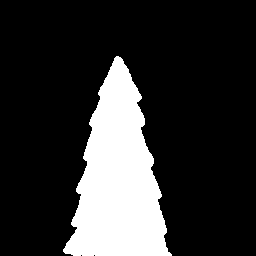
\includegraphics[width=\textwidth]{imagens/ex1/imageT1.png}
				\caption{}
                \label{fig:TransT1}
        \end{subfigure}
        ~
        \begin{subfigure}[b]{0.3\textwidth}
                
\includegraphics[width=\textwidth]{imagens/ex1/imageT2.png}
                \caption{}
                \label{fig:TransT2}
        \end{subfigure}
        ~
        \begin{subfigure}[b]{0.3\textwidth}
                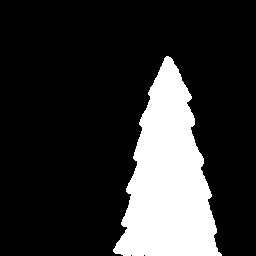
\includegraphics[width=\textwidth]{imagens/ex1/imageT3.png}
                \caption{}
                \label{fig:TransT3}       
        \end{subfigure}
        \caption{ \ref{fig:TransOriginal}. Image original
        \ref{fig:TransT1}. Imagem com translação verticalde 50 pixels
        \ref{fig:TransT2}. Imagem com translação horizontal  de 50 pixels
        \ref{fig:TransT3}. Imagem com translação vertical e horizontal de 50
        pixels}
        \label{fig:translacao}
\end{figure}

\subsection{Rotação}
A operação de rotação é uma tranformação geométrica que mapeia a posição de uma
forma em um espaço levando em consideração o ângulo desejado na transformação.
Todos os pontos da forma são rotacionados a partir de um ângulo constante em
relação ao ponto de rotação, para rotação no $\Re^2$, reta no $\Re^3$ ou
hiperplano para o $R^n$.
No $R^2$ os pontos de destino da forma podem ser calculados através das
seguintes equações:
\begin{align}
x'=cos(\theta)*(x_1-x_0)-sen(\theta)*(y_1-y_0)+x_0\\
y'=sen(\theta)*(x_1-x_0)+cos(\theta)*(y_1-y_0)+y_0\\
\end{align}
ou em termos matriciais.
\begin{align}
Im'=T*Im\\
Im'=\begin{bmatrix}
cos(\theta) & sen(\theta)\\
-sen(\theta) & cos(\theta)\\
\end{bmatrix}*
\begin{bmatrix}
x\\
y\\
\end{bmatrix}
\end{align}
Ao fazer uso da forma matricial deve-se perceber que a rotação ocorrerá somente
sobre a origem. Para contornar esta característica faz-se necessário o uso do
operador de translação, deslocando assim o ponto desejado para o centro das
coordenadas para só então realizar a rotação. Na figura \ref{fig:rotacao}
podemos ver o resultado da rotação.

\begin{figure}
		\centering
        \begin{subfigure}[b]{0.3\textwidth}
                
\includegraphics[width=\textwidth]{imagens/ex1/imageScale1.png}
                \caption{}
                \label{fig:RotOriginal}
        \end{subfigure}%
        ~ %add desired spacing between images, e. g. ~, \quad, \qquad, \hfill etc.
          %(or a blank line to force the subfigure onto a new line)
        \begin{subfigure}[b]{0.3\textwidth}
                
\includegraphics[width=\textwidth]{imagens/ex1/image30.png}
				\caption{}
                \label{fig:rot1}

        \end{subfigure}
        ~
        \begin{subfigure}[b]{0.3\textwidth}
                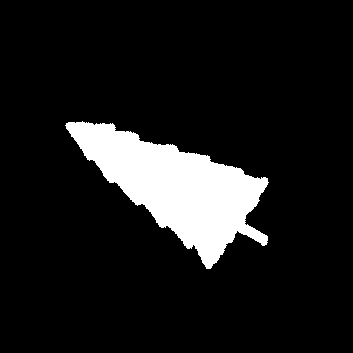
\includegraphics[width=\textwidth]{imagens/ex1/image60.png}
                \caption{}
                \label{fig:rot2}

        \end{subfigure}
        ~
        \begin{subfigure}[b]{0.3\textwidth}
                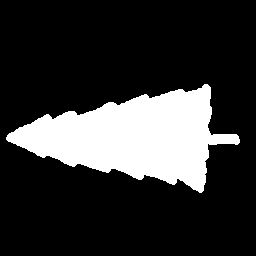
\includegraphics[width=\textwidth]{imagens/ex1/image90.png}
                \caption{}
                \label{fig:rot3}       
        \end{subfigure}
        \caption{ \ref{fig:RotOriginal}. Image original
        \ref{fig:rot1}. Imagem com rotação de 30º
        \ref{fig:rot2}. Imagem com rotação de 60º
        \ref{fig:rot3}. Imagem com rotação de 90º
        }
        \label{fig:rotacao}
\end{figure}


\subsection{Redimensionamento}
O redimensionamento é uma transformação linear que aumenta ou diminue o tamanho
de uma forma em um fator constante em todas as direções da forma. Normalmente
este aumento ou redução é feita de forma uniforme, mas pode ser feita de forma
diferente em cada eixo da representação da forma. Um fator de redimencionamento
maior que 1 reflete em um aumento na imagem, menor que 1 em uma redução e um
fator igual a 1 não é feita nenhuma tranformação. É importante ressaltar que
valores menor que 0 não são válidos.
Bem como as operações de translação e rotação o redimencionamento também pode
ser representado por um produto matricial. O redimensionamento de um vetor
$\overleftarrow{v}=(x,y,z)$ por um fator $f$ resulta em um vetor
$\overleftarrow{w}=(fx,fy,fz)$, representado matricialmente por:

\begin{align}
Im'=T*Im\\
 Im' = 
\begin{bmatrix}
f_x & 0 & 0  \\
0 & f_y & 0  \\
0 & 0 & f_z  \\
\end{bmatrix}*
\begin{bmatrix}
x\\
y\\
z\\
\end{bmatrix}
\end{align}

$f_x,f_y,f_z$ são os fatores de redimensionamento para cada dimensão do vetor.

\begin{figure}
		\centering
        \begin{subfigure}[b]{0.3\textwidth}
                
\includegraphics[width=\textwidth,scale=1]{imagens/ex1/imageScale1.png}
                \caption{}
                \label{fig:RedOriginal}
        \end{subfigure}%
        ~ %add desired spacing between images, e. g. ~, \quad, \qquad, \hfill etc.
          %(or a blank line to force the subfigure onto a new line)
        \begin{subfigure}[b]{0.3\textwidth}
                
\includegraphics[width=\textwidth,scale=1]{imagens/ex1/imageScale2.png}
                \caption{}
                \label{fig:Red2}
        \end{subfigure}
        ~
        \begin{subfigure}[b]{0.3\textwidth}
  				
\includegraphics[width=\textwidth,scale=1]{imagens/ex1/imageScale3.png}
                \caption{}
                \label{fig:Red3}   
        \end{subfigure}
        \caption{ 
        \ref{fig:RedOriginal}. Image original
        \ref{fig:Red2}. Redimensionamento com fator 1.5
        \ref{fig:Red3}. Redimensionamento com fator 2
        }
        \label{fig:redimensionamento}
\end{figure}

\section{Contrate, Brilho e Gama}
As técnicas de modificação de histograma são conhecidas como técnicas ponto-a-ponto, uma
vez que o valor de tom de cinza de um certo pixel após o processamento depende apenas de seu
valor original. Dentre as principais técnicas temos o ajuste de brilho,
contraste e gama.

\subsection{Brilho}
O Brilho é um atributo de percepção visual no qual determina a intensidade de
energia emitida ou refletida por uma fonte, O brilho é uma característica
importante pois é ela que determina se a quantidade de luz é perceptível pelos
sensores ou pela aplicação. O ajuste de intensidade do brilho é feito a partir
da seguinte equação:
\begin{align}
Im'(x,y) = Im(x,y) + b
\end{align}
onde b é o valor de ajuste do brilho.


\subsection{Contraste}
O contrate é um atributo que permite que objetos sejam discriminados dentro de
um mesmo campo visual. Dois objetos com intensidades semelhantes são
dificilmentes distinguidos por sensores como o olho humano. O ajuste no
contraste tem como princípio aumentar a diferença de intensidade entre os
objetos.

\begin{align}
Im'(x,y) = c * Im(x,y)
\end{align}
onde c é o valor de ajuste do contraste.

\begin{figure}
\centering
		\begin{tikzpicture}[domain=0:255,scale=0.015]
		\begin{scope}                           % scope environment
			\clip  (-50,-10) rectangle (320,320);
			\draw[->] (-0,0) -- (255,0) node[above] {$x$};
			\draw[->] (0,-0) -- (0,255) node[above] {$f(x)$};
			\draw[color=red, domain=0:137] plot (\x,1.5*\x + 50) node[right] {};
			\draw[color=red, domain=137:255] plot (\x,255) node[right] {$f(x) = x$};
		\end{scope}
		\end{tikzpicture}
		\caption{Função de mapeamento com brilho=50 e contraste=1.5}
\end{figure}
~
\begin{figure}
\centering
	\begin{tikzpicture}[domain=0:255,scale=0.015]
		\begin{scope}                           % scope environment
			\clip  (-50,-10) rectangle (320,320);
			\draw[->] (-0,0) -- (255,0) node[above] {$x$};
			\draw[->] (0,-0) -- (0,255) node[above] {$f(x)$};
			\draw[color=red, domain=20:122] plot (\x,2.5 * \x - 50) node[right] {};
			\draw[color=red, domain=122:255] plot (\x,255) node[right] {$f(x) = x$};
			\draw[color=red, domain=0:20] plot (\x,0) node[right] {};
		\end{scope}           
	\end{tikzpicture}
	\caption{Função de mapeamento com brilho=-50 e contraste=2.5}
\end{figure}

\subsection{Gama}
O gama, assim como o ajuste de contraste é utilizado para aumentar a diferença
de intensidade entre os objetos porem de forma não linear. A regulação do gama
pode ser feita com base na seguinte função.
\begin{align}
Im'(x,y) = c * Im(x,y)^\gamma
\end{align}
onde c é um fator de correção do gama e $\gamma$ é o fator de gama. O fator de
correção é importante pois geralmente o função descrita acima retorna valores
muito altos.
\begin{figure}
\centering
		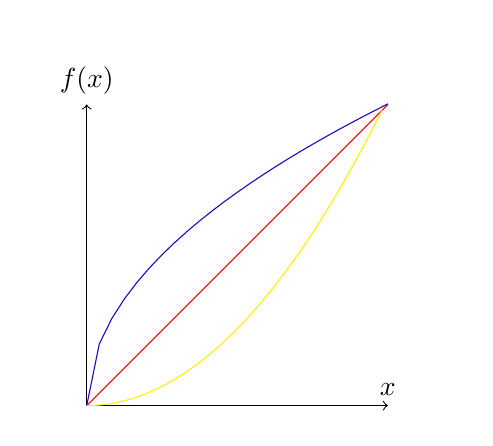
\begin{tikzpicture}[domain=0:255,scale=0.015]
		\begin{scope}                           % scope environment
			\clip  (-50,-10) rectangle (320,320);
			\draw[->] (-0,0) -- (255,0) node[above] {$x$};
			\draw[->] (0,-0) -- (0,255) node[above] {$f(x)$};
			\draw[color=red, domain=0:255] plot (\x,\x^1) node[above] { };
			\draw[color=blue, domain=0:255] plot (\x,16*\x^0.5) node[below] { };
			\draw[color=yellow, domain=0:25] plot ( 10 * \x, 0.4 * \x^2 ) node[above]{};
			
		\end{scope}
		\end{tikzpicture} 
		\caption{Função de mapeamento do gama. vermelho, azul e amarelo possuem 1,
		0,5 e 2 valores de gama respectivamente}
\end{figure}

\subsection{Resultado Obtidos}

\begin{figure} 
		\centering
		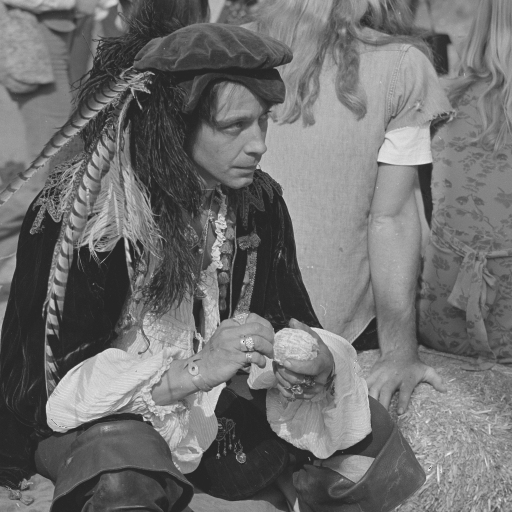
\includegraphics[width=0.3\textwidth,scale=1]{\matlabCodePath
		Trabalho_PDI/bd/pirate.png}
		\caption{Imagem utilizada como teste para as operação de brilho, contraste e
		gama}
		\label{fig:BrilhoContGamaOriginal}
\end{figure}

\begin{figure} 
		\centering 
		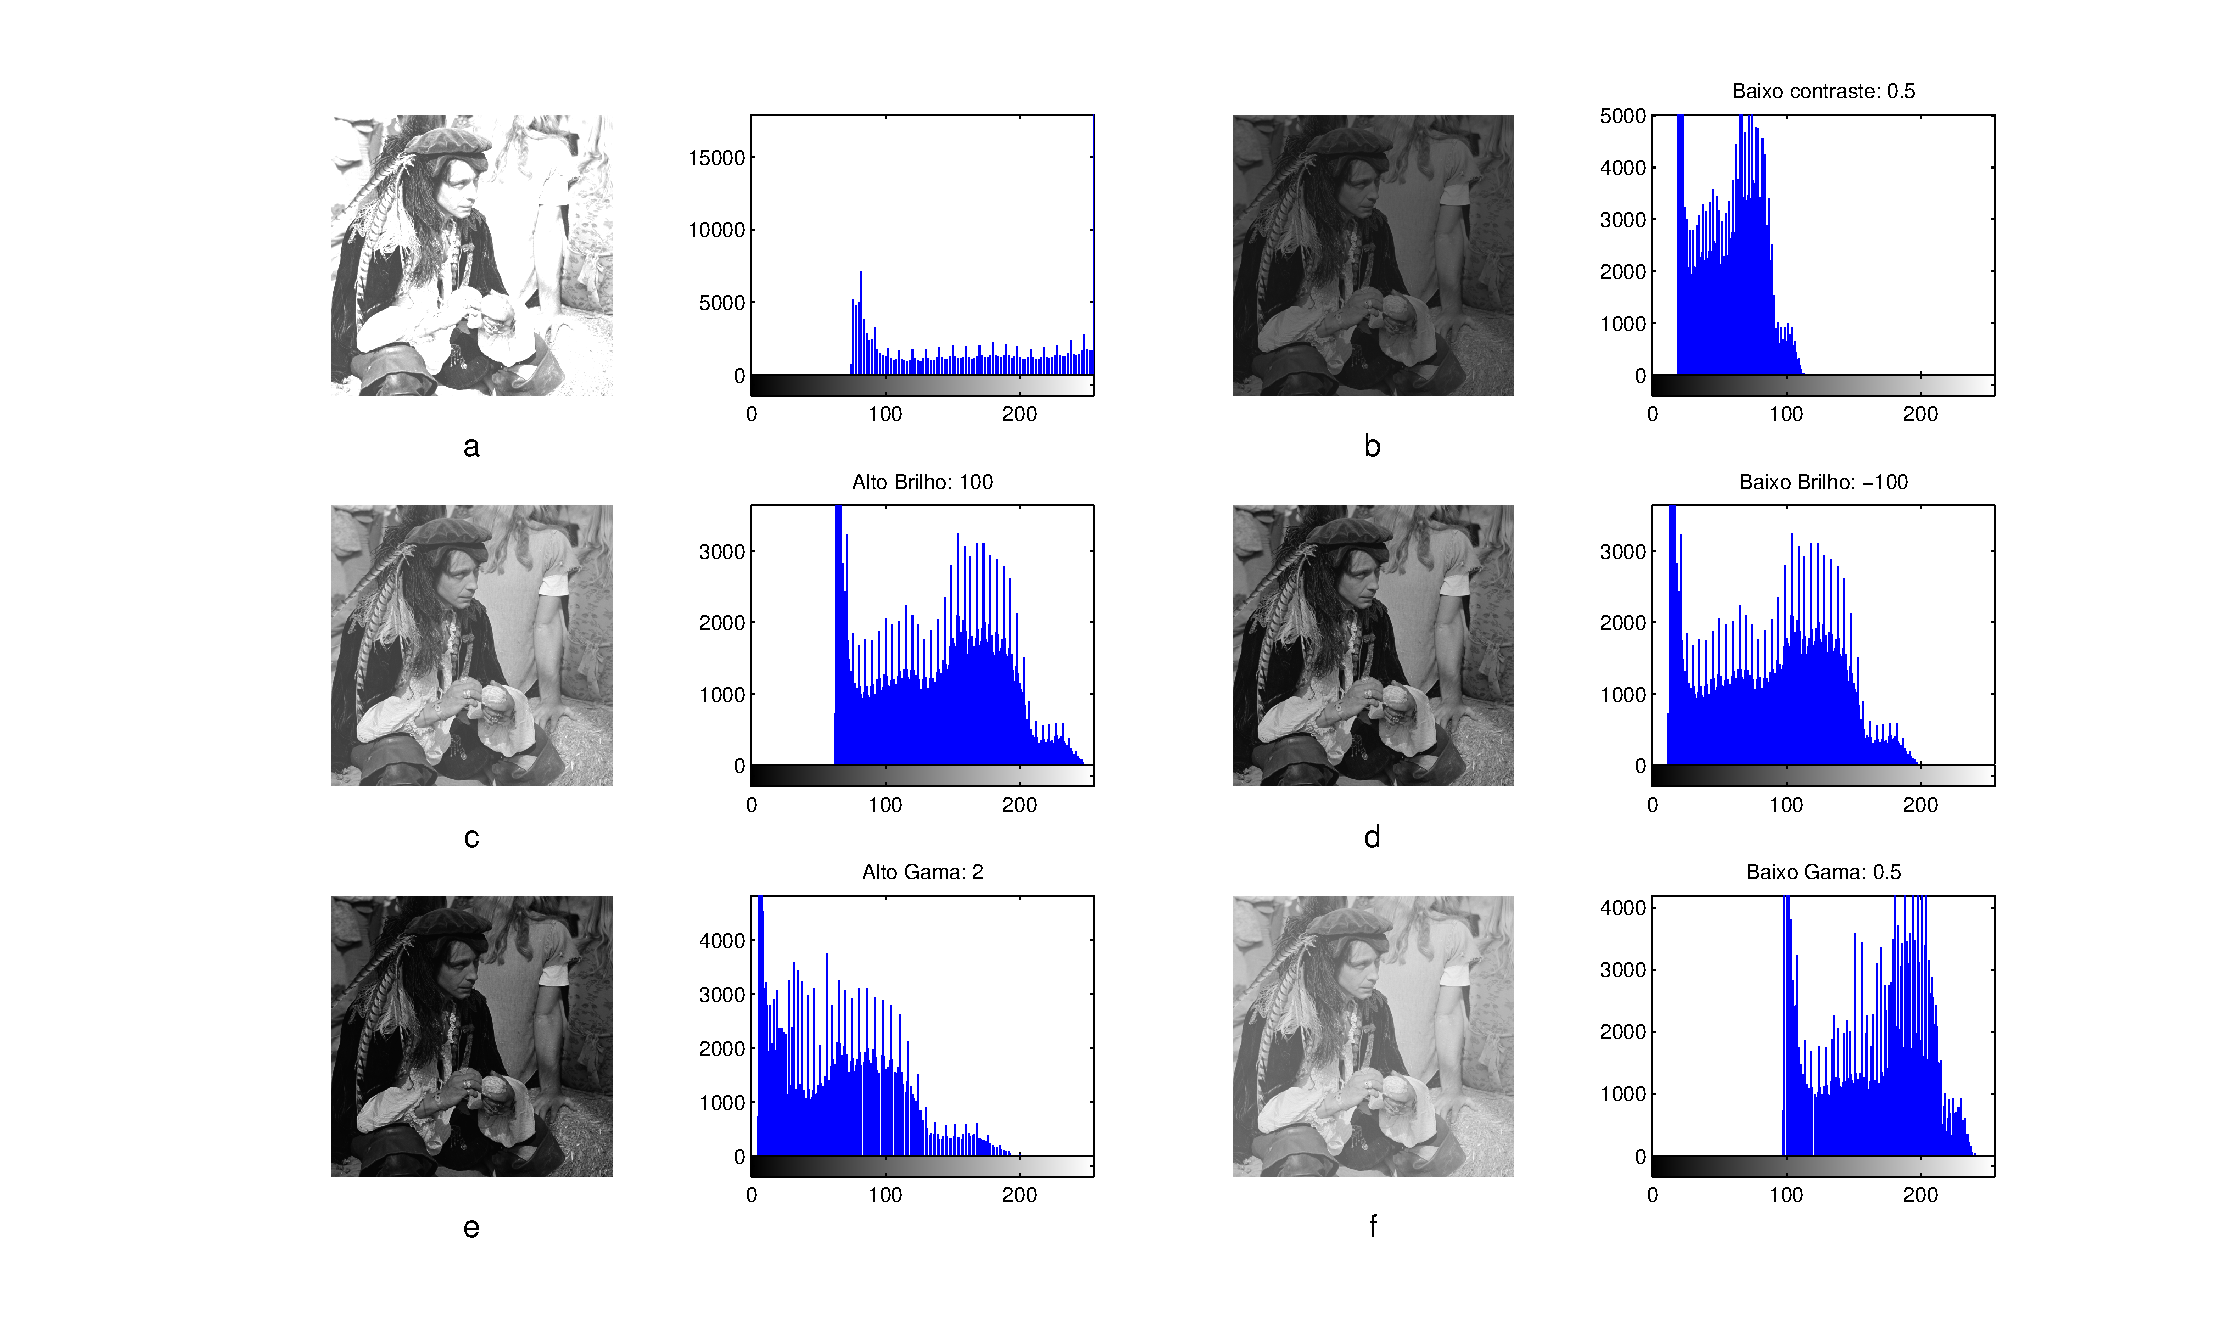
\includegraphics[width=\textwidth,scale=1, trim =
		4cm 0cm 0cm 1cm,clip]{\matlabCodePath
		Trabalho_PDI/q12/brilhoContrasteGama.eps}
		\caption{Resultado da aplicação das técnicas de ajuste de histograma.
		a)Contraste aplicado 2
		b)Contraste aplicado 0.5
		c)Brilho aplicado 25
		d)Brilho aplicado -25
		e)Gama aplicado 2
		f)Gama aplicado 0.5 
		}
		\label{fig:brilhContGamaRes}		
\end{figure}

Na figura \ref{fig:brilhContGamaRes} temos os resultados obtidos após a
realização de uma série de ajustes na figura \ref{fig:BrilhoContGamaOriginal}.
Podemos perceber através dos histogramas que a alteração do contraste
\ref{fig:brilhContGamaRes} a,b,  faz com que o hisograma seja alongado ou
comprimido ao longo dos possíveis valores da imagem. Diferentemente do ajuste
de contraste, o brilho apenas desloca o histograma,
figura \ref{fig:brilhContGamaRes} c,d. Caso o valor do brilho seja positivo o
histograma é deslocado para a região mas clara, caso negativo para a região mais
escura. O ajuste de gama,figura \ref{fig:brilhContGamaRes} e,f, é um pouco mais
peculiar que os dois anteriores. Por ser uma operação exponencial, caso o valor seja maior que 1 a imagem como um
todo terá a intensidade de seus pixels reduzidas, porém os pixels com valores de
intensidade menor serão ainda mais afetados pelo operador. caso o valor seja
menor que 1 a intensidade da imagem aumentará e da mesma forma os pixels com
valores de intensidade menor sofrerão maiores mudanças. O código fonte deste
exemplo pode ser visualizado no Apendice \ref{apend:contBriGama}


\section{Filtragem no domínio da frequência}
A transformada de Fourier é uma transformação matemática que permite que funções
possam ser expressas em componentes senoidais. O somatório destas componentes
tem como resultado a função orignal. A informação de frequencia destas
componentes são muito importantes tendo em vista que com elas podemos
identificar e filtrar ruídos que atuam em frequencias conhecidas. Também pode-se
fazer a filtragem de componentes de maiores ou menores frequencias a partir de
um limiar, filtros passa-baixa e filtros passa-alta respectivamente.

Para um sinal de uma dimensão temos a seguinte equação utilizada para calcular a
transforda de fourier de $s(t)$:
\begin{align}
S(f) = \int_{-\infty}^{\infty} s(t) \cdot e^{-i 2\pi f t} dt.
\end{align}
Para duas dimensões temos a seguinte equação:
\begin{align}
\displaystyle \hat{f}(\xi_x, \xi_y)=
\displaystyle \iint f(x,y) e^{-2\pi i(\xi_x x+\xi_y y)}\,dx\,dy
\end{align}

$\xi_x$ e $\xi_y$ são as frequências calculadas sobre a imagem.
À medida que nos aproximamos da origem da transformada, imagem calculada a
partir da equação anterior, as baixas frequências correspondem aos componentes
de intensidade de variação lenta em uma imagem como mudanças suaves de
intensidade na parede ou em outras regiões uniformes da imagem.
À medida que nos distanciamos da origem da transformada, as frequências mais
altas começam a corresponder a variações de intensidade cada vez mais rápidas
como bordas de objetos e outros elementos, figura
\ref{fig:lenaOriginalEspectro}.
De acordo com as características citadas anteriormente podemos contruir as
matrizes para a filtragem  no dominio da frequencia, figura
\ref{fig:filtrosFrequencia}. Uma das características do domínio da frequência é
que a filtragem espacial pode ser realizada utilizando apenas um produto de
matrizes. O resultado da filtragem pode ser visualizado na figura. O código
fonte utilizado encontra-se no Apêndice \ref{apend:filtragemCod}.


\begin{figure}
		\centering
        \begin{subfigure}[b]{0.3\textwidth}
                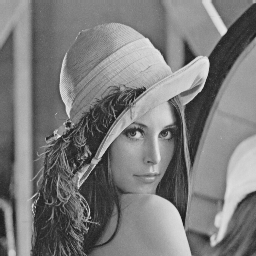
\includegraphics[width=\textwidth,scale=1]{imagens/ex2/lena.png}
                \caption{}
                \label{fig:lenaOriginal}
        \end{subfigure}%
        ~ %add desired spacing between images, e. g. ~, \quad, \qquad, \hfill etc.
          %(or a blank line to force the subfigure onto a new line)
        \begin{subfigure}[b]{0.3\textwidth}
                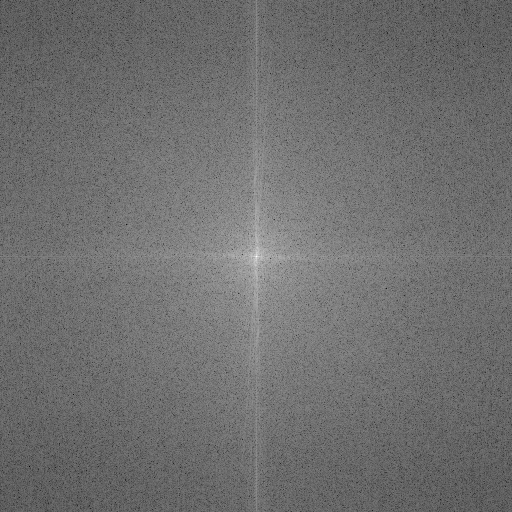
\includegraphics[width=\textwidth,scale=1]{\matlabCodePath Trabalho_PDI/q13-q14/espectroOriginal.png}
                \caption{}
                \label{fig:especOriginal}
        \end{subfigure}
       
        \caption{ 
        \ref{fig:lenaOriginal}. Image original
        \ref{fig:especOriginal}. Espectro de Fourier da imagem.
        }
		\label{fig:lenaOriginalEspectro}
\end{figure}

\begin{figure}
		\centering
        \begin{subfigure}[b]{0.3\textwidth}
                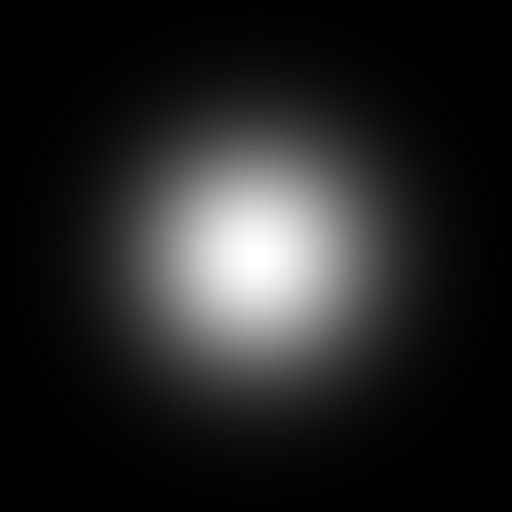
\includegraphics[width=\textwidth,scale=1]{\matlabCodePath Trabalho_PDI/q13-q14/passaBaixa.png}
                \caption{}
                \label{fig:passaBaixa}
        \end{subfigure}%
        ~ %add desired spacing between images, e. g. ~, \quad, \qquad, \hfill etc.
          %(or a blank line to force the subfigure onto a new line)
        \begin{subfigure}[b]{0.3\textwidth}
                
\includegraphics[width=\textwidth,scale=1]{\matlabCodePath Trabalho_PDI/q13-q14/passaAlta.png}
                \caption{}
                \label{fig:passaAlta}
        \end{subfigure}
       
        \caption{ 
        \ref{fig:passaBaixa}. Filtro passa baixa.
        \ref{fig:passaAlta}. Filtro passa alta. 
        }
	\label{fig:filtrosFrequencia}
\end{figure}

\begin{figure}
		\centering
        \begin{subfigure}[b]{0.3\textwidth} 
                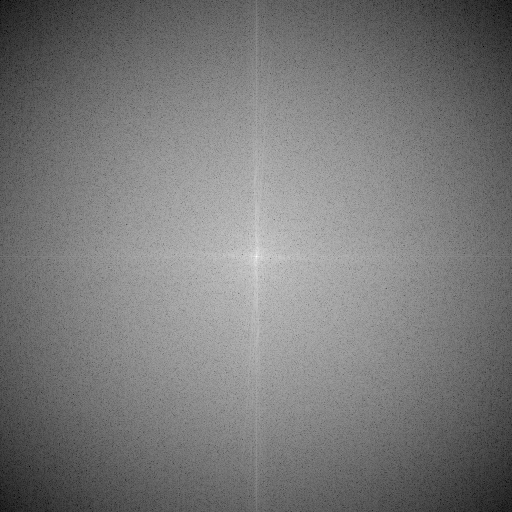
\includegraphics[width=\textwidth,scale=1]{\matlabCodePath Trabalho_PDI/q13-q14/filtradaPBSpec.png}
                \caption{}
                \label{fig:passaBaixa}
        \end{subfigure}%
        ~ %add desired spacing between images, e. g. ~, \quad, \qquad, \hfill etc.
          %(or a blank line to force the subfigure onto a new line)
        \begin{subfigure}[b]{0.3\textwidth}
                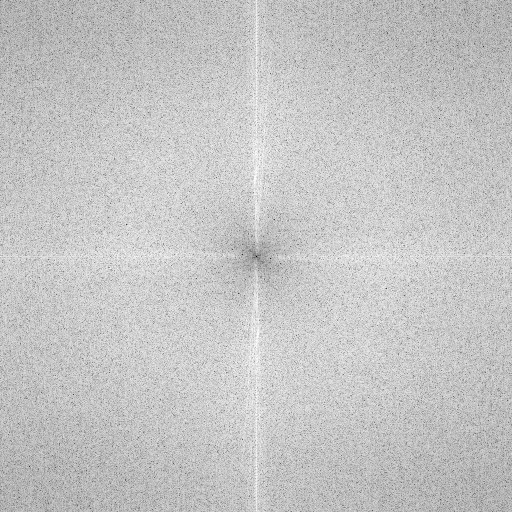
\includegraphics[width=\textwidth,scale=1]{\matlabCodePath Trabalho_PDI/q13-q14/filtradaPASpec.png}
                \caption{}
                \label{fig:passaAlta}
        \end{subfigure}
 		~      
		\centering
        \begin{subfigure}[b]{0.3\textwidth}
                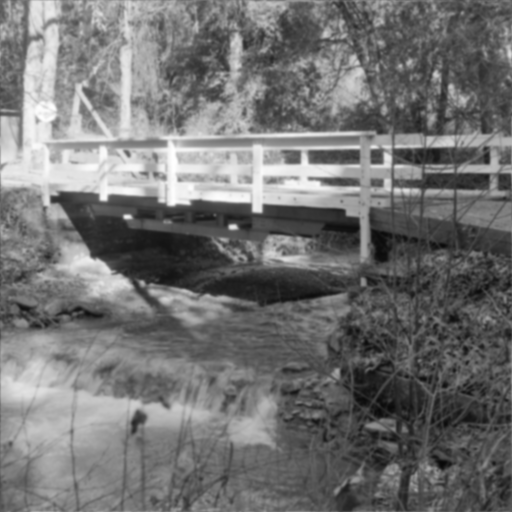
\includegraphics[width=\textwidth,scale=1]{\matlabCodePath Trabalho_PDI/q13-q14/filtradaPB.png}
                \caption{}
                \label{fig:passaBaixa} 
        \end{subfigure}%
        ~ %add desired spacing between images, e. g. ~, \quad, \qquad, \hfill etc.
          %(or a blank line to force the subfigure onto a new line)
        \begin{subfigure}[b]{0.3\textwidth}
                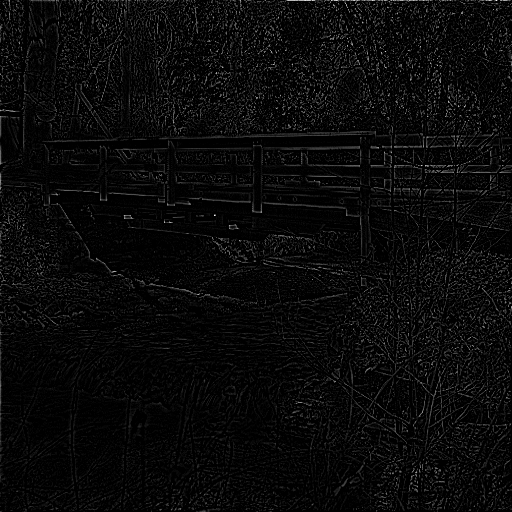
\includegraphics[width=\textwidth,scale=1]{\matlabCodePath Trabalho_PDI/q13-q14/filtradaPA.png}
                \caption{}
                \label{fig:passaAlta}
        \end{subfigure}      
      
        \caption{ 
        \ref{fig:passaBaixa}. Filtro passa baixa.
        \ref{fig:passaAlta}. Filtro passa alta.
        }
	\label{fig:filtrosFrequencia}
\end{figure}

\section{Segmentação Baseada em cores}

\subsection{Espaço de cores RGB}
O espaço de cores RGB é formado por todas as combinações possíveis das cores
R(Red), G(Green) e B(Blue), vermelho, verde e azul respectivamente. Esse espaço
de cores é normalmente representado por um cubo onde cada eixo representa uma
das componetes,ou canais, de cor, a intensidade de cada componente
indica a cor resultante, figura \ref{subfig:cuboRGB}.
Em imagens coloridas baseadas nesta representação o valor máximo de cada
componente é 255. Na figura \ref{fig:rgbComb} temos o resultado de algumas
combinações deste espaço de cores. Neste espaço de cores, vale ressaltar que a
cor branca é formada pela combinação da máxima intensidade de todas as três componentes, a cor preta
pela combinação da intensidade mínima das três componentes.


\begin{figure} 
		\centering
		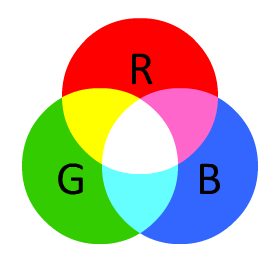
\includegraphics[width=0.3\textwidth,scale=1]{imagens/ex4/RGB_combinacao.png}
        \caption{Algumas combinações possíves do espaço de cores RGB. Perceba
        que na interseção das cores são produzidas cores diferentes.}
        \label{fig:rgbComb}
\end{figure}
        
        
\subsection{Espaço de cores HSV} 
O espaço de cores HSV também conhecido como HSB, assim como o RGB possue 3
componentes para representar as cores. As três componentes estão organizadas de forma que suas componentes
armazenem informação da matiz, saturação e brilho separadamente. O lugar
geométrico deste espaço de cores é um cilindro, as vezes também representado por
um cone, onde a altura é o nível de brilho, o raio a intensidade da cor e o
ângulo a cor no espectro luminoso, matiz.
A matiz, componente H, descreve a cor encontrada no espectro eletromagnético, é
dessa componente que descrevemos as cores eg. vermelho, verde, laranja. A
saturação, componente S, descreve a puresa da cor em relação a cor branca. Uma
cor totalmente impura, valor mínimo desta componente, tem como cor resultante a cor branca.
A última componente V ou B, o brilho, descreve quanta luz é emitida do objeto.
A conversão entre os espaços de cores HSV e RGB pode ser feita facilmente com os
seguintes comandos no Matlab. 


\begin{lstlisting}[frame=single, numbers=left]
	% Converter RGB para HSV 
	hsv_image = rgb2hsv(rgb_image)
	% Converter HSV para RGB
	rgb_image = hsv2rgb(hsv_image)
\end{lstlisting}

No Matlab, por padrão as imagens coloridas são alocadas em matrizes onde cada
canal representa uma das componentes do RGB. Cada elemento da matriz representa
uma componente de um pixel da imagem com valores variando entre [0, 255]. Após a
conversão da imagem para o formato HSV as matrizes de cada componente têm seus
valores variando entre [0, 1].

\begin{figure}
		\centering
        \begin{subfigure}[b]{0.3\textwidth}
                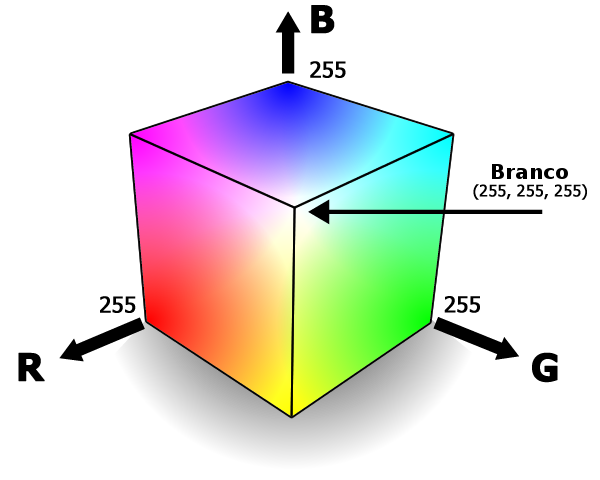
\includegraphics[width=\textwidth,scale=1]{imagens/ex4/rgbColorspace.png}
                \caption{}
                \label{subfig:cuboRGB}
                
        \end{subfigure}%
        ~ %add desired spacing between images, e. g. ~, \quad, \qquad, \hfill etc.
          %(or a blank line to force the subfigure onto a new line)
        \begin{subfigure}[b]{0.3\textwidth}
                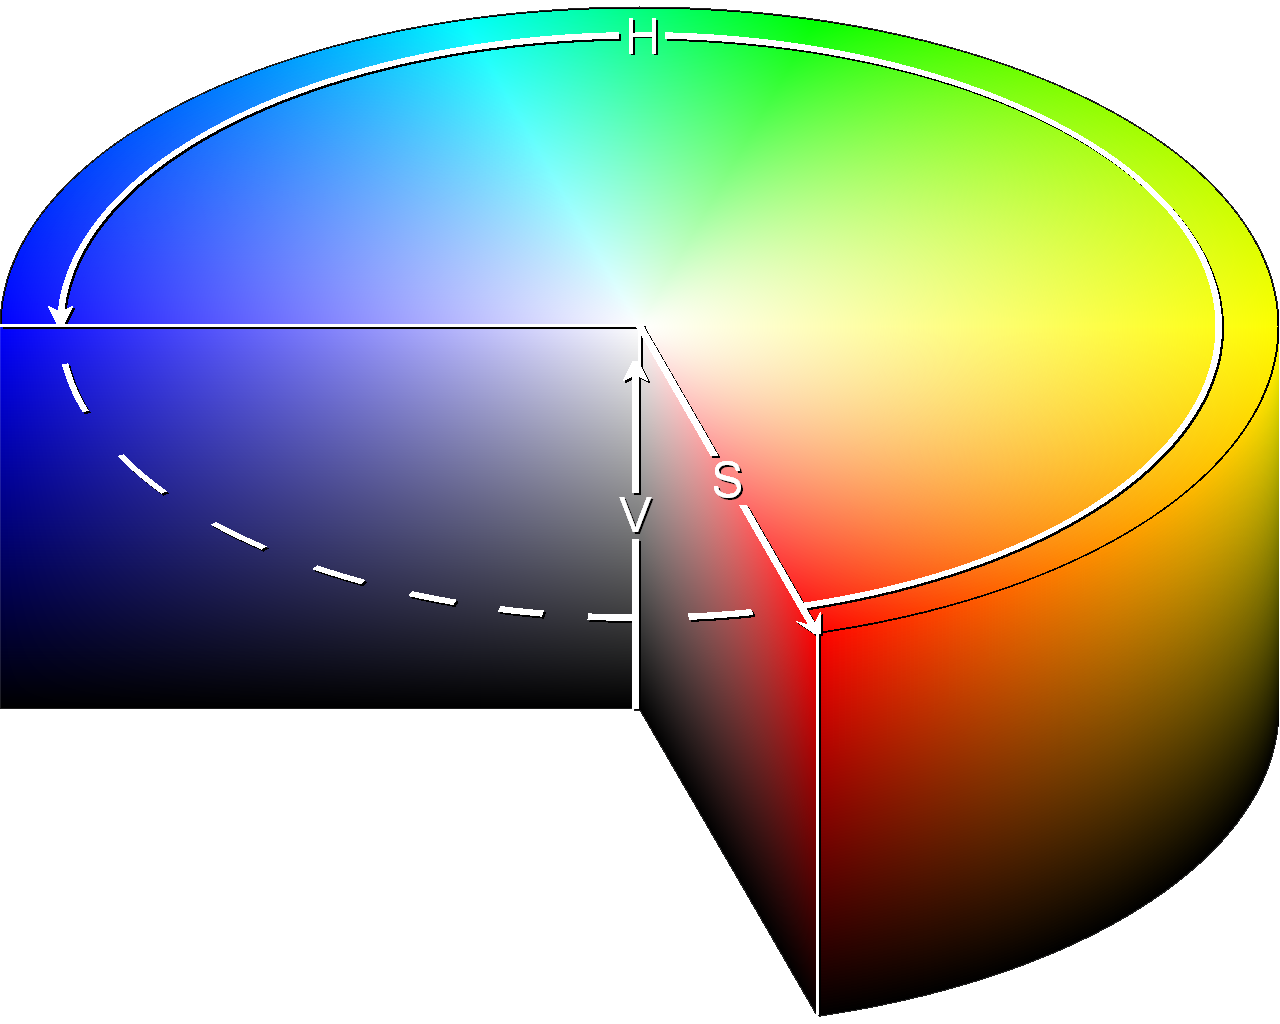
\includegraphics[width=\textwidth,scale=1]{imagens/ex4/HSVColorSpace.png}
                \caption{}
                \label{subfig:cilindoHSV}
        \end{subfigure}
        
        \caption{ 
        \ref{subfig:cuboRGB}. Representação do espaço de cores RGB
        \ref{subfig:cilindoHSV}. Representação do espaço de cores HSV.
        } 
	\label{fig:filtrosFrequencia}
\end{figure}

\subsection{Segmentação baseada na cor da pele}
A definição do limiar de segmentação baseado em cores é feita utilizando o
espaço de cores HSV. Como dito anteriormente este espaço de cores possui como
característica a separação da informação de cor de outras informações como
luminosidade e pureza. A figura \ref{fig:skinSegment}a foi utilizada para a
definição dos limiares. Foi verificado que os valores H que melhores descrevem
os tons da pele estão no intervalo [0 , 0.1], intervalo este que representa
10\% da faixa de valores possíveis do canal H. Foi verificado também que para o
canal S os valores que melhor representam o tom da pele estão na faixa de [0.4
1 0.8]. O resultado da combinação dos dois limiares em S e H com a imagem de
entrada pode ser visualizado na imagem \ref{fig:skinSegment}d.  O código
fonte utilizado encontra-se no Apêndice \ref{apend:skinSegment}.


\begin{figure} 
		\centering 
		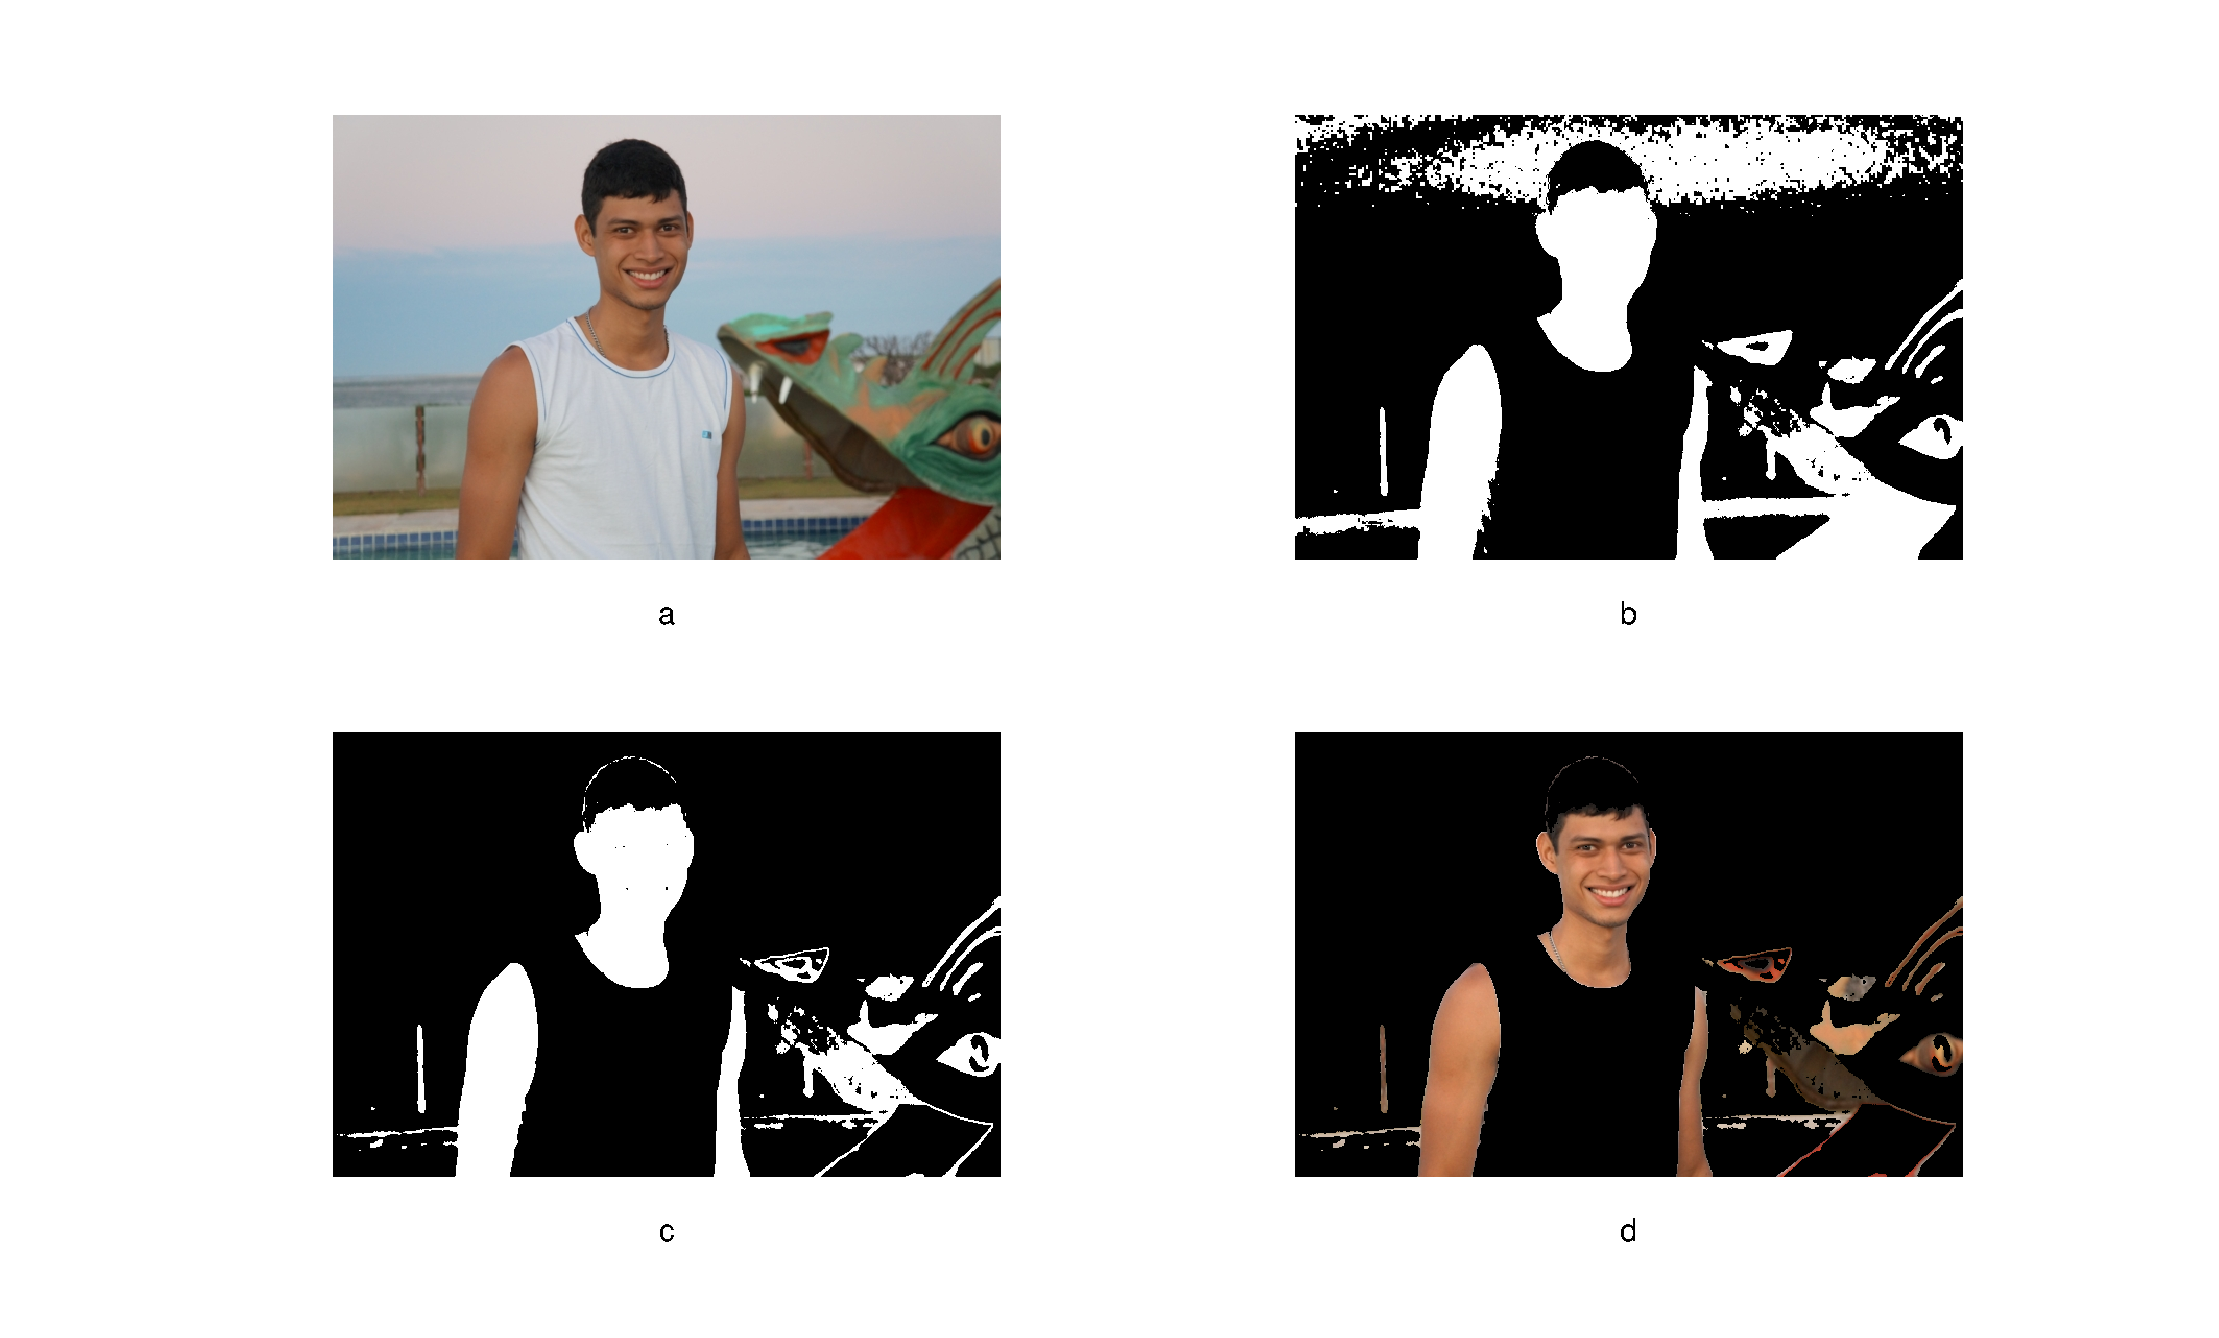
\includegraphics[width=\textwidth,scale=1, trim =
		4cm 0cm 0cm 1cm,clip]{\matlabCodePath
		Trabalho_PDI/skin/skinResult.eps}
		\caption{Resultado da aplicação das técnicas de segmentação.
		a)Imagem Original
		b)Filtro aplicado ao canal H.
		c)Filtro aplicado ao canal H e S
		d)Imagem resultante após os filtros.
		}
		\label{fig:skinSegment}		
\end{figure}

\subsection{Rastreamento baseado em cor}
\begin{figure} 
		\centering 
		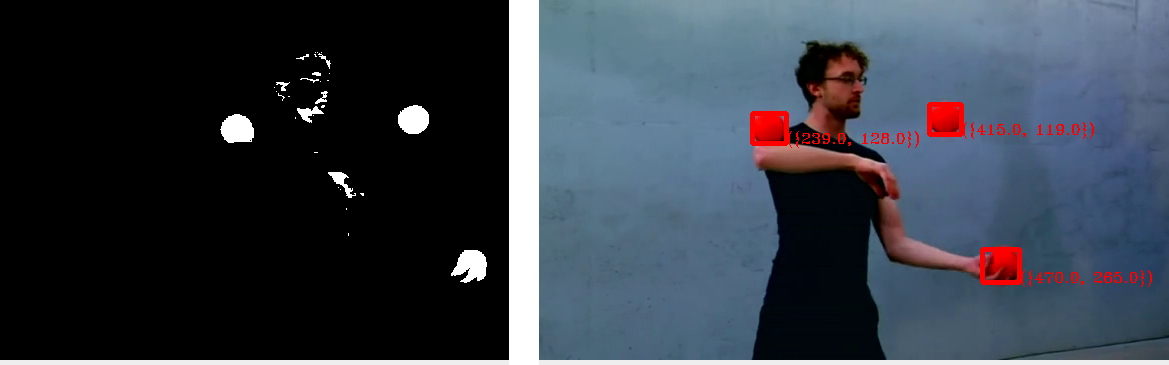
\includegraphics[width=\textwidth,scale=1, trim =
		4cm 0cm 0cm 1cm,clip]{imagens/track/redBall.png}
		\caption{Resultado da aplicação das técnicas de segmentação.
		a)Imagem Original
		b)Filtro aplicado ao canal H.
		c)Filtro aplicado ao canal H e S
		d)Imagem resultante após os filtros.
		}
		\label{fig:skinSegment}		
\end{figure}
% ---
% Finaliza a parte no bookmark do PDF, para que se inicie o bookmark na raiz
% ---
\bookmarksetup{startatroot}% 
% ---

% ---
% Conclusão
% ---
\section*{Considerações finais}
\addcontentsline{toc}{section}{Considerações finais}



\begin{citacao}

\end{citacao}


% ]  				% FIM DE ARTIGO EM DUAS COLUNAS
% ---

% ----------------------------------------------------------
% Referências bibliográficas
% ----------------------------------------------------------
\bibliography{pdi}
 
% ----------------------------------------------------------
% Glossário
% ----------------------------------------------------------
%
% Há diversas soluções prontas para glossário em LaTeX. 
% Consulte o manual do abnTeX2 para obter sugestões.
%
%\glossary

% ----------------------------------------------------------
% Apêndices
% ----------------------------------------------------------

% ---
% Inicia os apêndices
% ---
\begin{apendicesenv} 

% ----------------------------------------------------------
\chapter{Código fonte: Translação, Rotação e Redimensionamento}
\label{apend:transRotRed}

	
 	\lstset{extendedchars=true,inputencoding=utf8/latin1}
 	\lstinputlisting[frame=single,
 					 numbers=left]{\matlabCodePath
 	Trabalho_PDI/q11/topico11.m}



\chapter{Código fonte: Ajuste de Brilho, Contraste e Gama}
\label{apend:contBriGama}

\lstset{extendedchars=true,inputencoding=utf8/latin1}

\lstinputlisting[frame=single, numbers=left]{\matlabCodePath
Trabalho_PDI/q12/ajustaBrilho.m}
\lstinputlisting[frame=single, numbers=left]{\matlabCodePath
Trabalho_PDI/q12/ajustaContraste.m}
\lstinputlisting[frame=single, numbers=left]{\matlabCodePath
Trabalho_PDI/q12/ajustaGama.m}
\lstinputlisting[frame=single, numbers=left]{\matlabCodePath
Trabalho_PDI/q12/brilhoContraste.m}



\chapter{Código fonte: Filtragem no domínio da frequência}
\label{apend:filtragemCod}
\lstset{extendedchars=true,inputencoding=utf8/latin1}
\lstinputlisting[frame=single, numbers=left]{\matlabCodePath
Trabalho_PDI/q13-q14/filtragem.m}

\chapter{Código fonte: Segmentação de Pele}
\label{apend:skinSegment}
\lstset{extendedchars=true,inputencoding=utf8/latin1}
\lstinputlisting[frame=single, numbers=left]{\matlabCodePath
Trabalho_PDI/skin/skin.m}


\end{apendicesenv}
% ---

% ----------------------------------------------------------
% Anexos
% ----------------------------------------------------------
\cftinserthook{toc}{AAA}


% ---
% Inicia os anexos
% ---
%\anexos
%\begin{anexosenv}
%\chapter{}
%\end{anexosenv}

\end{document}
